\chapter{Adaptive time stepping}
\label{ch:p2}

\begin{keybox}
\textbf{Key idea.} Coarsening is multi-scale \emph{in time}: the
spinodal quench is stiff (interfaces form on a fast timescale that a
time integrator must resolve) and then coarsening slows down
geometrically. A single fixed time step cannot serve both regimes
efficiently. An \emph{error-controlled} step---small during the quench,
large through the tail---delivers a target accuracy at a fraction of the
cost. This chapter treats that claim as a \emph{measurement}: we verify
the integrator's order, build a reference solution, and report the
\emph{real} cost and the \emph{honest} speed-up.
\end{keybox}

\begin{keybox}
\textbf{Accuracy is measured against a reference, not read off the
energy.} A lower free energy does \emph{not} mean a more accurate
solution --- an integrator can reach a lower energy simply by taking a
different (even worse) trajectory. Throughout this chapter accuracy means
the error of $c(T)$ (and of the physics diagnostics: energy, structure-
factor length scale, phase fractions) against a tight small-$\Delta t$
\emph{reference}.
\end{keybox}

\section{The model and the integrator}

The equation is unchanged from Chapter~\ref{ch:p1}: the conserved
gradient flow \eqref{eq:ch} of the Ginzburg--Landau energy \eqref{eq:F}.
What changes is the time integration. A backward-difference formula (BDF)
of order $p$ writes the time derivative at $t_{n+1}$ as
%
\begin{equation}
  \dd{c}{t}\Big|_{t_{n+1}} \approx \frac{1}{\Delta t_n}\Big(c_0\,c^{n+1}
  - \sum_{j\ge1} c_j\,c^{n+1-j}\Big),
  \label{eq:bdf}
\end{equation}
%
turning each step into a nonlinear (Newton) solve. Here we use $p=2$.

\paragraph{The variable-step BDF2, mapped to code.} A constant-coefficient
BDF2 ($c_0=\tfrac32$, weights $[2,-\tfrac12]$) is only second-order when
the step is \emph{constant}. Under an adaptive $\Delta t$ the step ratio
$r=\Delta t_n/\Delta t_{n-1}$ varies, so the coefficients must be rebuilt
from the actual $(\Delta t_n,\Delta t_{n-1})$ every step. In
\file{cahn\_hilliard.step} this is exactly
%
\begin{equation}
  c_0 = \frac{1+2r}{1+r},\qquad
  [\,c_1,\,c_2\,] = \Big[\,1+r,\; -\frac{r^2}{1+r}\,\Big],\qquad
  \sigma=\frac{c_0}{\Delta t_n},
  \label{eq:vbdf2}
\end{equation}
%
which for $r=1$ collapses to the constant-step $\tfrac32,[2,-\tfrac12]$
scheme bit-for-bit (so fixed-$\Delta t$ trajectories are unchanged). The
\textbf{startup} is handled by the same code: the first step (and any
step taken before a previous step exists) falls back to BDF1
($c_0=1$, $[c_1]=[1]$), whose single $O(\Delta t^2)$ local error does not
spoil the global second order. A \textbf{rejected} step rewinds the state
\emph{including} $\Delta t_{n-1}$, so the replayed, halved step rebuilds
\eqref{eq:vbdf2} consistently. We \emph{verify} this claim below rather
than asserting it.

\paragraph{Step-doubling error control.} From a state $c^n$, take one step
of size $\Delta t$ to get $c_{\Delta t}$, and \emph{separately} two steps
of $\Delta t/2$ to get $c_{\Delta t/2}$. Their difference estimates the
local truncation error (relative $L_2$ form, robust to the sharpest
interface node),
%
\begin{equation}
  \text{LTE} \;\approx\; \frac{\lVert c_{\Delta t} - c_{\Delta t/2}\rVert_2}
  {(2^{p}-1)\,\lVert c_{\Delta t/2}\rVert_2}.
\end{equation}
%
Accept the (more accurate) half-step solution if $\text{LTE}<\text{tol}$,
and propose the next step from the standard controller
%
\begin{equation}
  \Delta t_{\text{new}} = \Delta t \cdot \mathrm{clamp}\!\Big(
  \text{safety}\,(\text{tol}/\text{LTE})^{1/(p+1)},\;\tfrac12,\;2\Big);
\end{equation}
%
otherwise \emph{reject}, halve $\Delta t$, and retry (Wodo \&
Ganapathysubramanian, JCP 230 (2011) 6037). Each \emph{attempt} therefore
costs \textbf{one full plus two half solves}; this is the cost we account
for honestly below.

\section{Step 1 --- verify the integrator on a smooth problem}

Before trusting an integrator on the chaotic quench, verify its
\emph{observed order} on a problem whose exact solution is smooth in time.
We use a single low-$k$ cosine, $c=a\cos(2\pi x)$ with small amplitude
$a$ --- a Neumann eigenmode ($k=2\pi$) --- with $\kappa k^2>1$, so it
\emph{relaxes}
smoothly (exponential single-mode decay). Refining $\Delta t$ against a
fine-$\Delta t$ reference on the \emph{same} mesh (so spatial error
cancels) and reading the slope with the shared convergence diagnostic
gives
%
\begin{equation*}
  \text{BDF1: observed order } \PtwoOrderBDFone, \qquad
  \text{BDF2: observed order } \PtwoOrderBDFtwo,
\end{equation*}
%
i.e.\ first and second order as designed (Fig.~\ref{fig:p2order}). This
is the evidence that the variable-step BDF2 of \eqref{eq:vbdf2} is
implemented correctly; only now do we use it on the quench.

\begin{figure}[h]\centering
  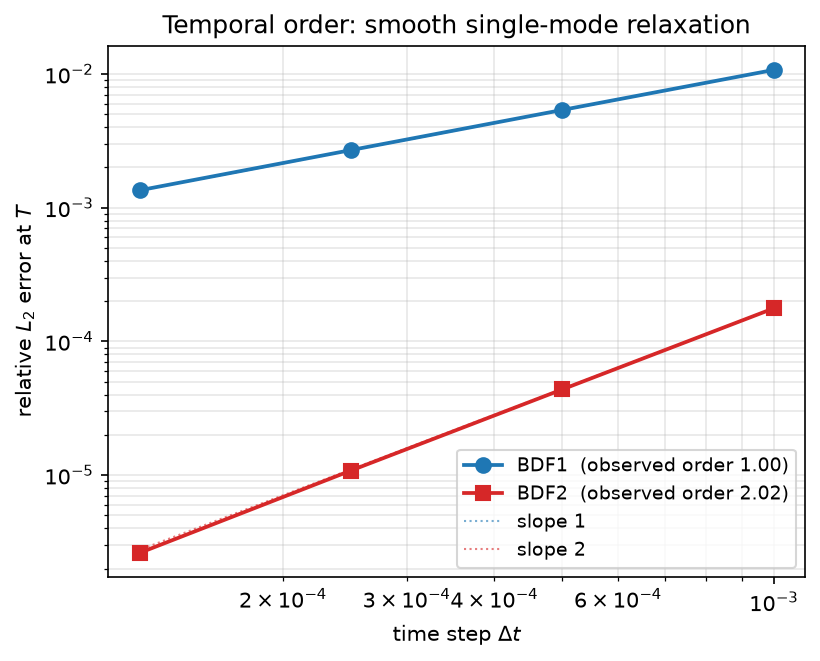
\includegraphics[width=0.66\linewidth]{figures/p2_order.png}
  \caption{Temporal-order verification on the smooth single-mode
    relaxation: the relative $L_2$ error at $T$ versus $\Delta t$, with
    reference slopes 1 and 2. BDF1 tracks slope~1, BDF2 tracks slope~2.}
  \label{fig:p2order}
\end{figure}

\section{Step 2 --- a reference, and the stiffness cliff}

We march the binary quench ($\PtwoSide\times\PtwoSide$, sharp interface
$\kappa=\PtwoKappa$, to $t=\PtwoTend$) and build a \emph{reference} by
integrating with a tight fixed step $\Delta t=\PtwoRefdt$
($\PtwoRefsteps$ steps). We check the reference against itself by halving
$\Delta t$: the change in $c(T)$ is $\PtwoRefselfcheck$ (relative
$L_2$), so the reference is converged to well below the errors we compare
against.

Refining a \emph{fixed} step toward the reference, the error falls at the
expected order (observed order $\PtwoFixedOrder$) --- \emph{until} the
step is too large to resolve the quench, at which point the morphology is
destroyed (the ``stiffness cliff''). A comfortable fixed step
$\Delta t=\PtwoSafedt$ ($\PtwoSafesteps$ steps) sits safely below the
cliff (relative $L_2$ error $\PtwoSaferelL$), but pushing to
$\Delta t=\PtwoCliffdt$ lands \emph{above} it and the error jumps to
$\PtwoCliffrelL$ --- more than an order of magnitude worse.
\textbf{This is the real reason a fixed step is awkward:} you must know
the quench's stiffness in advance to choose it, and a step safe for the
quench is wastefully small for the coarsening tail.

\section{Step 3 --- the adaptive run, with real cost}

The controller finds the stiff phase on its own: the accepted step
collapses to $\Delta t_{\min}=\PtwoDtmin$ through the spinodal onset and
grows to the ceiling $\Delta t_{\max}=\PtwoDtmax$ through coarsening ---
several orders of magnitude (Fig.~\ref{fig:p2dt}, top). We report the
\emph{real} cost, not the accepted-step count alone
(Table~\ref{tab:p2cost}): at $\text{tol}=\PtwoTol$ the run takes
$\PtwoAccepted$ accepted and $\PtwoRejected$ rejected steps; with one
full and two half solves per attempt that is $\PtwoFull$ full and
$\PtwoHalf$ half solves, $\PtwoNewton$ Newton/linear solves in total, and
$\PtwoWall$\,s of wall time. Its accuracy against the reference is
relative $L_2 = \PtwoAdrelL$, free-energy error $\PtwoAdFerr$, and a
structure-factor length scale of $\PtwoAdlam$ cells, matching the
reference's $\PtwoReflam$. The energy trajectory is indistinguishable
from the reference at a fraction of the steps (Fig.~\ref{fig:p2energy}).

\begin{figure}[h]\centering
  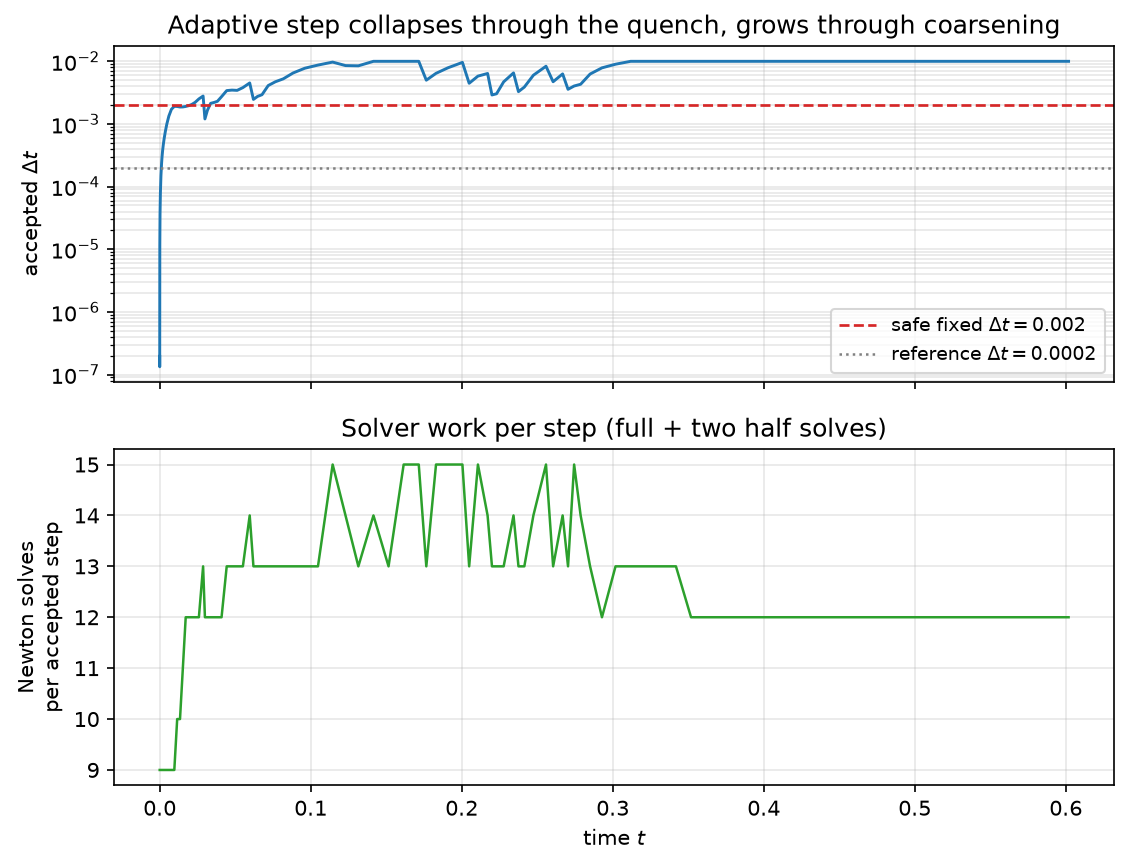
\includegraphics[width=0.82\linewidth]{figures/p2_dt_newton.png}
  \caption{Top: the accepted step size collapses through the quench
    (below even the reference step) and grows by orders of magnitude
    through coarsening; the safe fixed step (dashed) must stay small the
    whole time. Bottom: Newton solves per accepted step (full $+$ two
    half solves) --- the solver works hardest through the stiff onset.}
  \label{fig:p2dt}
\end{figure}

\begin{keybox}
\textbf{Robust statistics vs the pixel field.} Two integrators that take
different step \emph{sequences} produce different \emph{coarsened
patterns} (which domain merges when is chaotically sensitive), exactly as
changing the RNG seed does in Chapter~\ref{ch:p1}. So the pixelwise
$c(T)$ error has a floor set by this sensitivity, while the
\emph{physics} --- free energy, structure-factor length scale, phase
fractions --- agrees to much tighter tolerance
(Fig.~\ref{fig:p2morph}). Report both, and lean on the robust statistics.
\end{keybox}

\section{Step 4 --- convergence, the knee, and the honest speed-up}

Sweeping the tolerance over $\PtwoNtols$ values, the error against the
reference reaches its minimum near $\text{tol}=\PtwoKneeTol$ and does
\emph{not} improve for tighter tolerances --- indeed at this level it is
non-monotone, sitting on a trajectory-sensitivity floor of order
$10^{-3}$ in relative $L_2$ --- even as the cost keeps climbing
(Fig.~\ref{fig:p2conv}). That minimum is the \textbf{accuracy--cost
knee}: the tolerance worth using; tightening further is wasted work.

\paragraph{Matched-accuracy speed-up.} The honest comparison holds
\emph{accuracy} fixed and compares cost. To reach the adaptive run's
$c(T)$ accuracy with a \emph{fixed} step requires $\PtwoMatchedSteps$
steps ($\approx\PtwoMatchedSolves$ solves), versus the adaptive run's
$\PtwoAccepted$ accepted steps ($\PtwoNewton$ solves): a matched-accuracy
saving of $\PtwoSpeedupSteps\times$ in steps and $\PtwoSpeedupSolves\times$
in solves (the step-doubling overhead of three solves per step is why the
solve saving is smaller than the step saving). For contrast, the naive
worst-case bound --- a fixed step \emph{pinned} at the quench's smallest
adaptive step for the whole horizon --- would need $\PtwoWorstImplied$
steps; that number overstates the case and we do \emph{not} claim it as
the speed-up.

\begin{figure}[h]\centering
  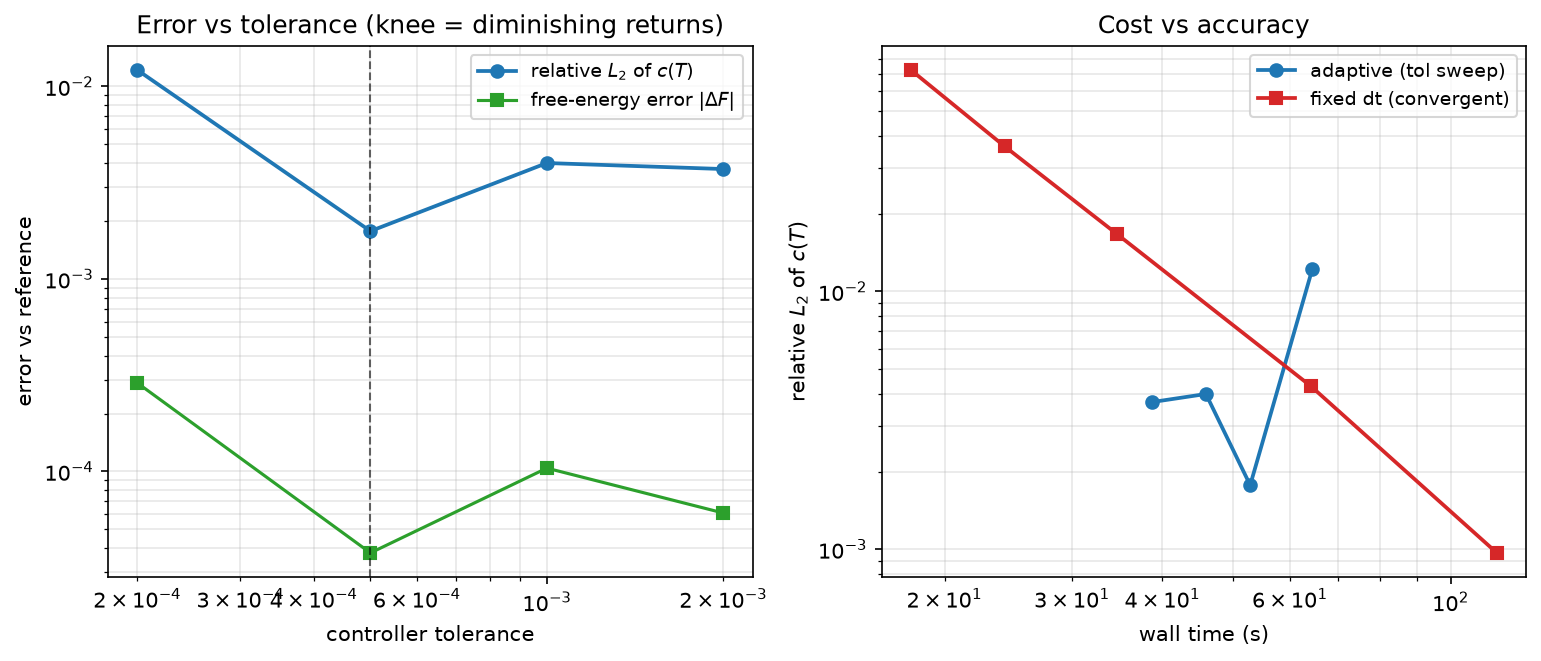
\includegraphics[width=\linewidth]{figures/p2_convergence.png}
  \caption{Left: error vs controller tolerance --- the pixelwise $L_2$
    error and the free-energy error both fall, then flatten at the knee
    (dashed). Right: accuracy vs wall time for the adaptive tolerance
    sweep and the convergent fixed-$\Delta t$ sweep.}
  \label{fig:p2conv}
\end{figure}

\begin{figure}[h]\centering
  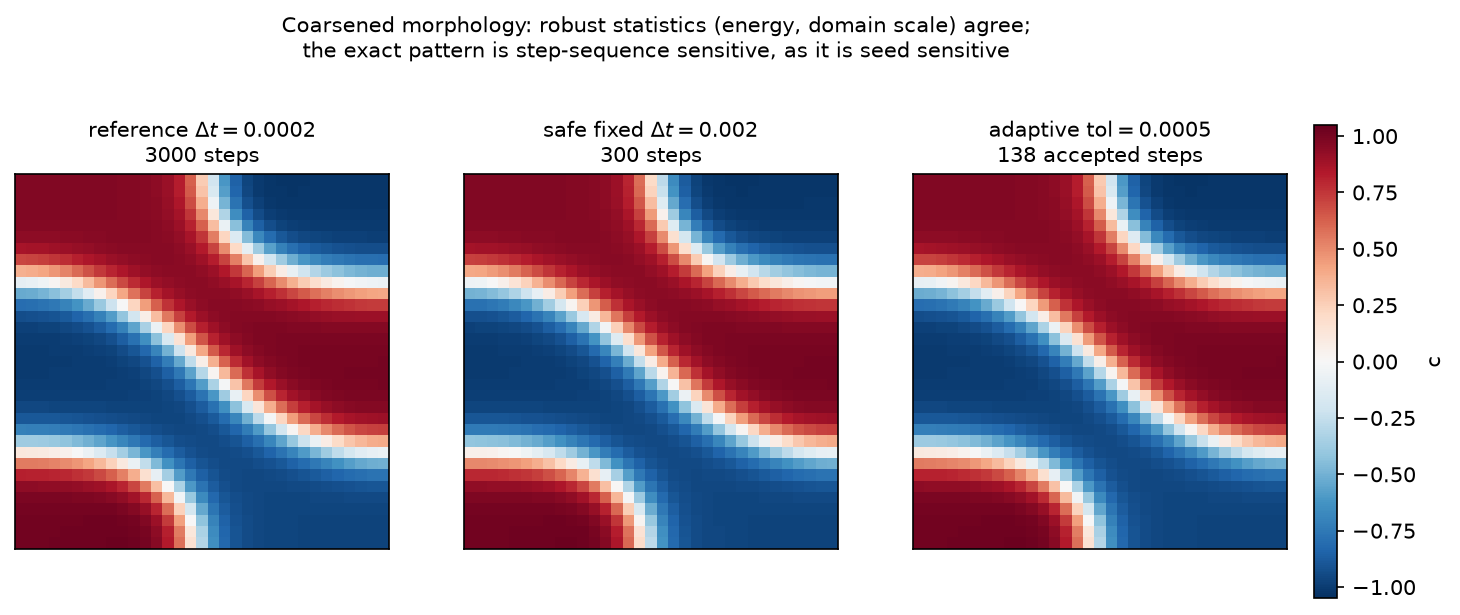
\includegraphics[width=\linewidth]{figures/p2_morphology.png}
  \caption{Final coarsened morphology from the reference, the safe fixed
    step, and the adaptive run. The robust statistics (energy, domain
    scale) agree; the exact pattern is step-sequence sensitive, as it is
    seed sensitive.}
  \label{fig:p2morph}
\end{figure}

\begin{figure}[h]\centering
  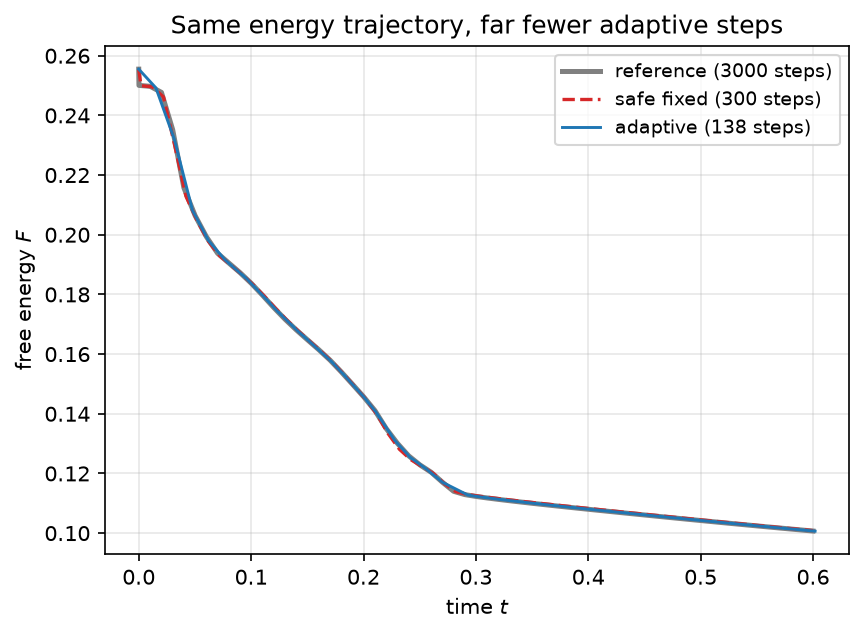
\includegraphics[width=0.66\linewidth]{figures/p2_energy.png}
  \caption{Free-energy history: the adaptive run (few accepted steps)
    traces the same $F(t)$ as the tight reference and the safe fixed
    step. Energy alone cannot rank accuracy --- that is why we compare
    against the reference, not by ``whose energy is lower''.}
  \label{fig:p2energy}
\end{figure}

\begin{table}[h]\centering
\caption{Real cost of the adaptive run (tol $=\PtwoTol$) and the
  matched-accuracy fixed alternative. Solves are total Newton/linear
  solves; the adaptive attempt cost is one full plus two half solves.}
\label{tab:p2cost}
\small
\begin{tabular}{lcc}
\toprule
 & adaptive & matched fixed \\
\midrule
accepted steps            & \PtwoAccepted & \PtwoMatchedSteps \\
rejected steps            & \PtwoRejected & --- \\
full / half solves        & $\PtwoFull$ / $\PtwoHalf$ & --- \\
total Newton/linear solves & \PtwoNewton & $\approx\PtwoMatchedSolves$ \\
$\Delta t$ range          & $\PtwoDtmin \to \PtwoDtmax$ & fixed \\
wall time (s)             & \PtwoWall & --- \\
\midrule
rel.\ $L_2$ of $c(T)$     & \multicolumn{2}{c}{$\PtwoAdrelL$ (matched)} \\
free-energy error         & \multicolumn{2}{c}{$\PtwoAdFerr$} \\
\bottomrule
\end{tabular}
\end{table}

\section{Run it}

\begin{runbox}
\textbf{Run it (the workflow).}
\begin{lstlisting}
cd physics/02_ch_adaptive_stepping
python run_harness.py --config configs/p2.yaml --mode quick \
    --output outputs/p2 --overwrite      # <2 min smoke
python run_harness.py --config configs/p2.yaml --mode reference \
    --output outputs/p2 --overwrite      # the cited numbers
python gen_figures.py --run outputs/p2   # figures + numbers/p2.tex
\end{lstlisting}
The harness writes \file{results.json} (checked against
\file{baseline.yaml}), \file{history.npz}, \file{metadata.json} and the
resolved config; \file{gen\_figures.py} renders every figure and the
number macros above \emph{purely} from that saved run.
\end{runbox}

\section{Code walk-through}

\paragraph{1. Verify, then use.} \code{order\_study} marches the smooth
cosine mode at several $\Delta t$ and reads the observed order with
\code{diagnostics.convergence.observed\_order}; only then does the harness
run the quench.

\paragraph{2. The adaptive march, instrumented.}
\begin{lstlisting}
from diffsim.physics.cahn_hilliard import adaptive_march
ts, dts = adaptive_march(stepper, t_end, tol=5e-4,
                         dt_max=1e-2, dt_min=1e-7)
\end{lstlisting}
\code{adaptive\_march} owns the accept/reject ladder and returns the
accepted $(t,\Delta t)$ pairs. The harness wraps \code{stepper.step} to
count \emph{every} solve, so it can reconstruct accepted vs.\ rejected
attempts and the per-step Newton work (each attempt is one full $+$ two
half solves) --- the honest cost in Table~\ref{tab:p2cost}.

\paragraph{3. Accuracy from a reference.} \code{\_metrics} compares each
run's $c(T)$ to the tight reference by relative $L_2$ \emph{and} by the
physics diagnostics (energy, structure-factor length scale, phase
fractions) --- never by ``whose energy is lower''.

\section{Explore on your own}

\question{Move the tolerance across the knee (\code{work\_tol}). Below the
knee the pixelwise error stops falling while the solve count keeps
rising --- confirm this, and explain it in terms of the
trajectory-sensitivity floor and the reference.}

\question{Widen the interface (increase $\kappa$). Does the stiffness
cliff move to a \emph{larger} safe fixed $\Delta t$? Relate the cliff
location to the fastest spinodal growth rate $\lambda_{\max}\!\sim\!
M/(4\kappa)$ and hence to the smallest step the controller must take.}

\question{Lengthen the horizon (\code{t\_end}) and raise \code{dt\_max}.
The coarsening tail tolerates ever-larger steps; does the
matched-accuracy speed-up grow? Why does adaptivity pay off more the
longer (and more scale-separated) the run?}

\question{Change the RNG seed and rerun. Which reported quantities move
(pixel field, domain scale, energy, phase values) and which do not?
Relate this to the seed discussion in Chapter~\ref{ch:p1} and to the
pixelwise-error floor.}

\question{Turn the controller off by using the largest fixed step above
the cliff. What does the morphology look like, and which diagnostic
(energy, length scale, phase fraction) flags the failure most clearly?}

% ====================================================================
